\documentclass[12pt]{report}

%% Language and font encodings
\usepackage[francais]{babel}
\usepackage[utf8]{inputenc}
\usepackage[T1]{fontenc}
\usepackage{lmodern} 
\usepackage[svgnames]{xcolor}
\usepackage{float} % figure
\usepackage{eurosym} % euro character
\usepackage{minted} % syntax coloring

%% Sets page size and margins
\usepackage[a4paper,top=3cm,bottom=2cm,left=3cm,right=3cm,marginparwidth=1.75cm]{geometry}

%% Useful packages
\usepackage{amsmath}
\usepackage{graphicx}
\usepackage[colorinlistoftodos]{todonotes}
\usepackage[colorlinks=true, allcolors=blue]{hyperref}

\title{Projet Licence ADSILLH 2017/2018\\Rapport}
\author{Gautier DELACOUR\\Pierre-Antoine ROUBY\\David TABARIE} % PA: TODO add GNOME-Music

\begin{document}
\maketitle

\begin{abstract}
Ce document présente les différents travaux effectués dans le cadre du projet sous licence libre de la licence ADSILLH.

\end{abstract}

\tableofcontents

% David: Suggestion: mettre des "\part" en lieu et place des chapters, ça nous permettrai d'avoir les titres sur une page entière. (?)
\chapter{Introduction}

\section{La Licence ADSILLH}
% from: http://dept-info.labri.fr/ENSEIGNEMENT/adsillh/contenu.html
L'objectif est de former des techniciens en informatique de haut
niveau en administration des systèmes d'information, polyvalents et
aptes à effectuer l'intégration de composants logiciels libres
appartenant à de nombreux domaines fonctionnels:

systèmes d'exploitation
bases de données
serveurs web
téléphonie logicielle

alliant ainsi de solides compétences d'administration à des capacités
de développement, en partant des couches les plus basses jusqu'aux
plus hautes, et l'aptitude à intégrer ces développements au sein des
communautés libres. Ce profil est explicitement recherché par les
entreprises et fait l'unicité de la formation. Il est couramment
appelé « DevOps Engineer ».

La formation apporte également des aspects organisationnels en droit
et en économie des logiciels libres.

\section{Le projet}
Le but du projet est avant tout de nous accoutumer au développement
collaboratif, et de nous apprendre à intéragir avec une communauté.

\chapter{Le projet GNOME}
% from: https://fr.wikipedia.org/wiki/GNOME
GNOME, acronyme de GNU Network Object Model Environment, est un
environnement de bureau libre convivial dont l'objectif est de rendre
accessible l'utilisation du système d'exploitation GNU au plus grand
nombre ; cette interface est actuellement populaire sur les systèmes
GNU/Linux et fonctionne également sur la plupart des systèmes de type
UNIX.

GNOME est développé par The GNOME Project dont les participants sont
bénévoles ou rémunérés par des entreprises externes au projet. La
majorité du travail est fournie par les contributeurs professionnels,
en premier lieu ceux travaillant pour Red Hat.
% PA: TODO add screen shot ?

\section{Les outils collaboratif du projet GNOME} 
% TODO PA: Cette partie a besion d'une relecture ;)
\subsection{Bugzilla}
\label{bugzilla}
% from: https://fr.wikipedia.org/wiki/Bugzilla
Bugzilla est une solution de gestion de bug, distribuer sous tri-licence 
MPL/GNU GPL/GNU LGPL, elle est developper et utilisé à l'origine par Mozilla.
GNOME a mis en place un \href{https://bugzilla.gnome.org}{bugzilla} pour 
la gestion des bug dans les differents porjet 
(figure~\ref{figure_bugzilla} page~\pageref{figure_bugzilla}).
\newline
% from: https://bugzilla.gnome.org/page.cgi?id=points.html
Buzilla integre aussi une fonctionnalité de "score" (figure~\ref{figure_bugzilla_score} 
page~\pageref{figure_bugzilla_score}), le but a l'origine et d'avoir une idée 
aproximative de l'activité d'une personne  sur le bugzilla, et donc 
des personnes qui sont le plus experimenté pour aidée les autres 
utilisateurs. Mais se dispositif s'est revelé peut éfficace. Le
score est donc plus une fonctionnalite rigolote qu'un vrai outils.
A noté qu'il existe quand même un classement de la semaine 
\href{https://bugzilla.gnome.org/page.cgi?id=weekly-bug-summary.html}{ici}.
% PA: Bonjour, j'ai utilisé le mot "rigolote" en 2017, vais-je finir en enfer ?
% PA: Nan en vrai j'ai pas trouvé mieux, si quelqu'un trouve mieux TODO

\subsection{Wiki}
\label{wiki}
GNOME dispose d'un \href{https://wiki.gnome.org/}{wiki} ou l'on peut retrouver 
les documentations sur les differents projets (figure~\ref{figure_wiki} page~\pageref{figure_wiki}).

\subsection{Git}
\label{git}
\label{cgit}
Le projet GNOME dispose de plusieurs interface Git. L'interface 
principal est baser sur le logiciel libre "cgit" (figure~\ref{figure_cgit} 
page~\pageref{figure_cgit}), on peut y retrouver la plupare des projets GNOME 
(\href{https://git.gnome.org/}{ici}). Pour créer un bug il faut passer par Bugzilla (section~\ref{bugzilla}).

\label{gitlab}
GNOME a aussi mit en place un \href{https://gitlab.gnome.org/GNOME}{GitLab} 
ou l'on peut trouver de nombre projet. L'interface est plus moderne 
et a la fason github nous pouvont créer de "PoolRequest" et la création 
de bug est simplifier car nous pouvons le créer sur la même interface 
(figure~\ref{figure_gitlab} page~\pageref{figure_gitlab}).

\label{github}
Il existe aussi un mirroir des repertoires git des projets 
\href{https://github.com/GNOME}{GNOME sur GitHub}.
% PA: TODO add screenshot ?

\subsection{IRC}
% PA: TODO Si quel qu'un a un peut utilisé l'irc de GNOME je veut bien qu'il écrive un truc

\subsection{Newcomers}
% PA: TODO ...

\newpage
\section{GNOME-Music}
% TODO GNOME-Music

\newpage
\section{GNOME Games}
GNOME Games est une application permettant la gestion d'une
bibliothèque vidéoludique. Elle est capable de s'interfacer avec de
nombreux émulateurs.
Au debut du projet Games étais disponible sur le git (section~\ref{cgit}) de GNOME, mais 
depuis peut il a étais migret sur le gitlab (section~\ref{gitlab}) du projet GNOME.

\subsection{Architecture du projet}
\subsubsection{Les projets assosié}
Le projet s'appuis sur plusieur autre projet:
\begin{itemize}
\item retro-gtk : Développé pas le mainteneur de Games et utilisant les bibliotheques libretro,
retro-gtk permet a Games de lancer les jeux retro (des jeux fait pour une ancienne console de jeux)
\item libmanette : Libmannette et aussi développé pas le mainteneur de Games. Cette bibliotheque permet
la gestion des manettes.
% TODO Verifier les info pour libmanette et retro-gtk 
\end{itemize}

% PA: On garde sa ?
% TODO Sondage
%          Oui | Non
% David:       |
% Gautier:     |
% PA:          | X
%----------------------
% result:   0  | 1
\subsubsection{Les sources}
Structure des sources du projet:
\begin{itemize}
\item data : contient toutes les données graphiques de l'application.
\item flatpak : contient tous les fichiers nécessaires à l'exécution de Flatpack.
\item plugins
\begin{itemize}
\item desktop : contient les fichiers s'occupant de la gestion du bureau.
\item dreamcast, game-cube, playstation... :  contient les fichiers gérant l'émulation des différentes consoles.
\end{itemize}
\item po
\item src
\begin{itemize}
\item command
\item core
\item database
\item dummy
\item event
\item gameinfo
\item gamepad
\item generic
\item grilo
\item retro
\item tracker
\item ui : contient les fichiers qui gèrent l'interface graphique.
\item utils
\end{itemize}
\item tools
\end{itemize}

\subsubsection{Hierarchy}


\subsection{Le langage Vala}
% from: https://fr.wikipedia.org/wiki/Vala_(langage)
Vala est un langage de programmation compilé, dont l'objectif est de
fournir les bénéfices des langages de programmation modernes (comme la
POO) aux développeurs de la plateforme GNOME qui utilisent GLib et son
système GObject.

Sa syntaxe est basée sur celle de C\# mais il ne nécessite pas
d'environnement d'exécution. Vala est transformé en code C, lui-même
compilé en code machine natif. Les avantages d'une telle chaîne de
compilation sont de produire des logiciels qui requièrent moins de
mémoire vive et qui s'exécutent plus rapidement.

De plus, ce passage par l'étape C rend possible l'utilisation des
bibliothèques C au moyen d'interfaces définies dans les fichiers
Vapi. Des fichiers Vapi sont fournis avec Vala pour une grande partie
de la plateforme GNOME, ainsi que pour d'autres bibliothèques.

\subsection{Le format Flatpak}
% from: https://fr.wikipedia.org/wiki/Flatpak
Flatpak, nommé xdg-app jusqu’en mai 2016, est un système de
virtualisation d’application pour les distributions GNU/Linux de
bureau.

L'objectif est de fournir un environnement « bac à sable » (sandbox)
sûr, isolé du reste du système, dans lequel les utilisateurs peuvent
exécuter des applications non validées par les dépôts de la
distribution (des versions de test, par exemple). Les applications
utilisent des appels de fonctions spécifiques fournies par xdg-app
pour contrôler les périphériques matériels ou accéder aux fichiers de
l'utilisateur, et xdg-app demande à l'utilisateur sa permission avant
de donner accès.

Le nom originel vient de freedesktop.org, qui est souvent abrégé en «
xdg », cette structure ayant hébergé sur ses serveurs le projet
xdg-app. En mai 2016, le projet a été rebaptisé « Flatpak ».

En juin 2016, un certain nombre d'applications connues sont portées en
format Flatpak, comme MonoDevelop, GNOME Shell, Pitivi ou LibreOffice.

Les applications Flatpak se téléchargent sous forme d'un fichier qui
peut s’exécuter directement sur le système, de façon indépendante de
la distribution linux précise utilisée, sous réserve que le logiciel
Flatpak ait été préalablement installé sur cette distribution.

Pour permettre au « bac à sable » de fonctionner malgré son isolement
du système, il faut donc que les bibliothèques ou dépendances
indispensables à un logiciel soient embarquées avec lui au sein de son
paquet « Flatpak ». Ce système a pour inconvénient d'embarquer
potentiellement plusieurs fois la même bibliothèque (une par paquet
Flatpak), et donc de prendre plus de place. Il a par contre pour
avantage de ne pas déstabiliser un logiciel Flatpak lors d'une mise à
jour de dépendances ou de bibliothèques, puisque cette mise à jour ne
le concernera pas. Il est dès lors assez simple de faire cohabiter
plusieurs versions d'un même logiciel.

\subsection{Découverte du logiciel}
\subsubsection{Compilation}
Nous avons rencontrés de nombreux problèmes relatifs à la compilation,
cela étant en grande partie du à l'utilisation de librairies encore en
état de développement actif, ainsi qu'au système de configuration
``Meson'' qui est un remplacement de ``./configure''.

Ainsi il a été nécessaire de compiler certaines librairies, parmis
lesquelles\footnote{Comme OS, nous avons utilisé Debian Sid}:
\begin{itemize}
\item retro-gtk
\item libmanette
\end{itemize}

% Gautier : installation compliquée -> versionnage + aucun fichier d'installation
% + problème d'affichage : les jeux sont chargés avec de mauvaises images
% + problème configuration : on ne peut pas configurer les touches du clavier dans les jeux
% + code pas commenté : possibilité de le commenter pour qu'il soit plus clair et plus accessible

\subsection{Bug reports}
% Gautier : système de statuts -> aucune explication
% Gautier : lecture de différents bug reports, et réécriture plus simple dans un fichier partagé pour effectuer un premier tri

\subsection{Patch}
% TODO PA: Cette partie a besion d'une relecture ;)
\subsubsection{Mise à jour du fichier HACKING}
Le premier patch (\href{http://bugzilla.gnome.org/show_bug.cgi?id=788692}{ici}) 
que nous avons envoyer, est en reponse a un bug repport, il ajouter une 
aide pour la compilation du projet. \newline
Il n'y avais aucune aide ou information dans la documentation sur la compilation
du projet. Etant nouveaux dans le projet GNOME nous n'avion pas connaisance de 
GNOME-Builder qui permet assez simplement de construire le projet. Mais
même avec cette outils la compilation c'est revéler ardu. En effet 
le fonctionement de Builder a tendence a changer entre les version et certain
action comme un 'git pull' peuvent posser problème.
Nous avons donc modifier le fichier HACKING du projet pour y ajouter des 
instruction de compilation. Le projet utilise pour le moment le système 
'autotools' pour sa compilation, mais il est prevu pour la version 2.30, 
qu'il passe sous un system avec le logiciel 'meson' pour la configuration. 
\newline
Nous avons donc nous même recontré de nombreux problème de compilation 
il nous a donc semblé important de donnée des indications pour que les 
prochaines personne qui voudrais contribuer ne sois pas frenné par un 
probleme comme celui-ci.
Il y a eu de nombre ajustement demandé par le mainteneur et le patch n'a 
pas encore étais aprouvé. \newline

\subsubsection{Mise à jour du fichier README.md}
Le second patch (\href{http://bugzilla.gnome.org/show_bug.cgi?id=790454}{ici}) 
que nous avons envoyer, est une mise a jour de la documentation de retro-gtk, 
en effet retro-gtk et passais d'un système de compilation 'autotools' a un
système avec le logiciel 'meson' et le compilateur 'ninja'.
Nous avons donc mis a jour le fichier README.md en respectant la syntax
'Marckdown', utilisé par github et gitlab par exemple.
Le patch n'a pas encore étais aprouvé. \newline

\subsubsection{Retoure a la collection avec les touches Alt+Left}
% TODO PA: David ?

% Annexe:
\appendix
\chapter{GNOME en images}

\begin{figure}[p]
  % from: https://bugzilla.gnome.org
  \caption{\label{figure_bugzilla} Le bugzilla du projet GNOME}
  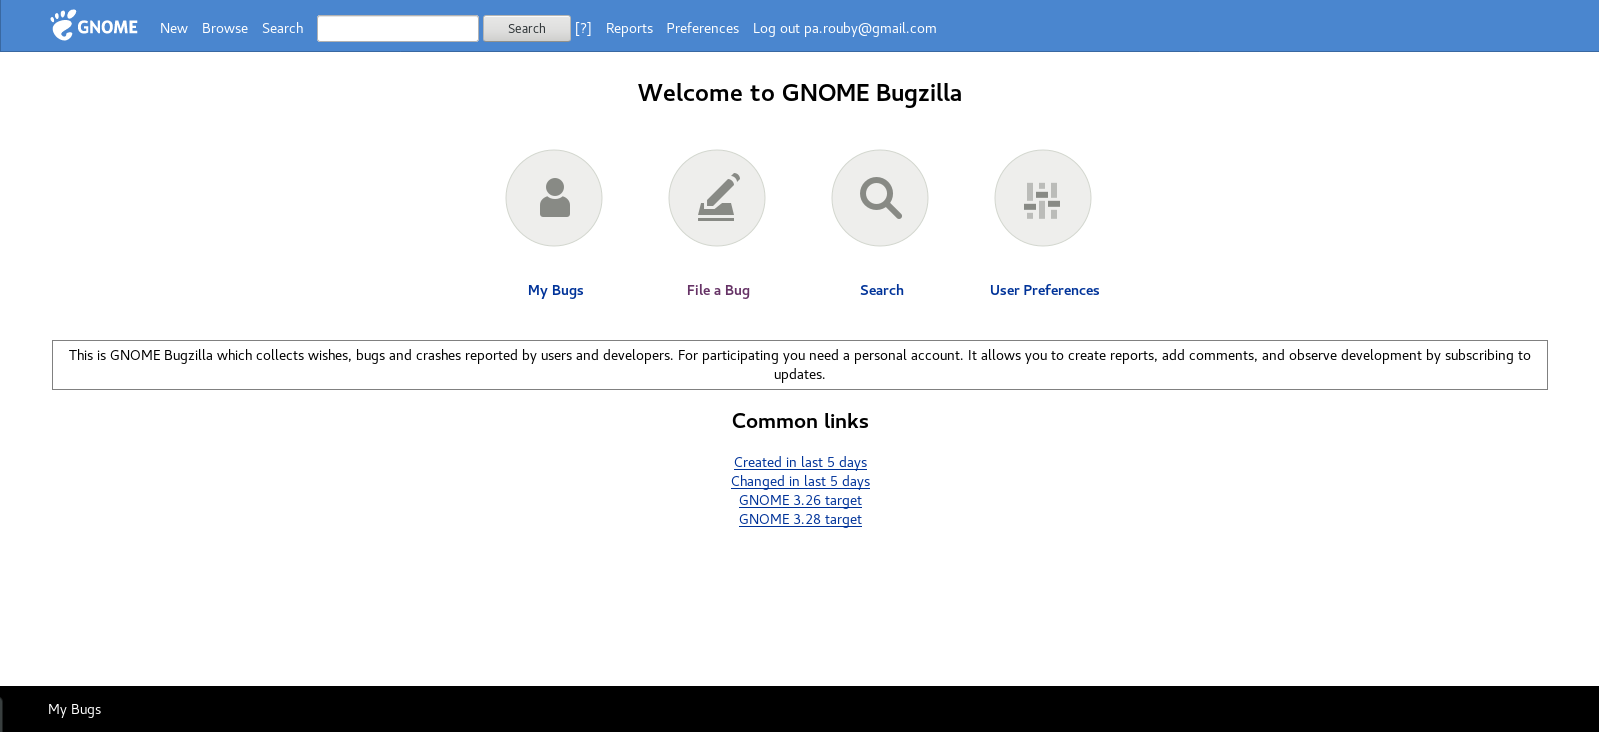
\includegraphics[width=15cm]{images/bugzilla_gnome_org.png}
\end{figure}

\begin{figure}[p]
  % from: https://bugzilla.gnome.org
  \caption{\label{figure_bugzilla_score} Score sur bugzilla}
  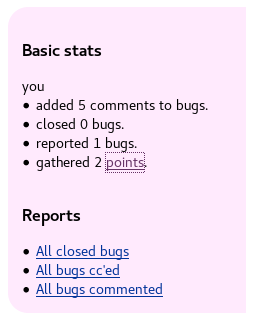
\includegraphics[width=5cm]{images/score.png}
\end{figure}

\begin{figure}[p]
  % from: https://wiki.gnome.org
  \caption{\label{figure_wiki} Le wiki du projet GNOME}
  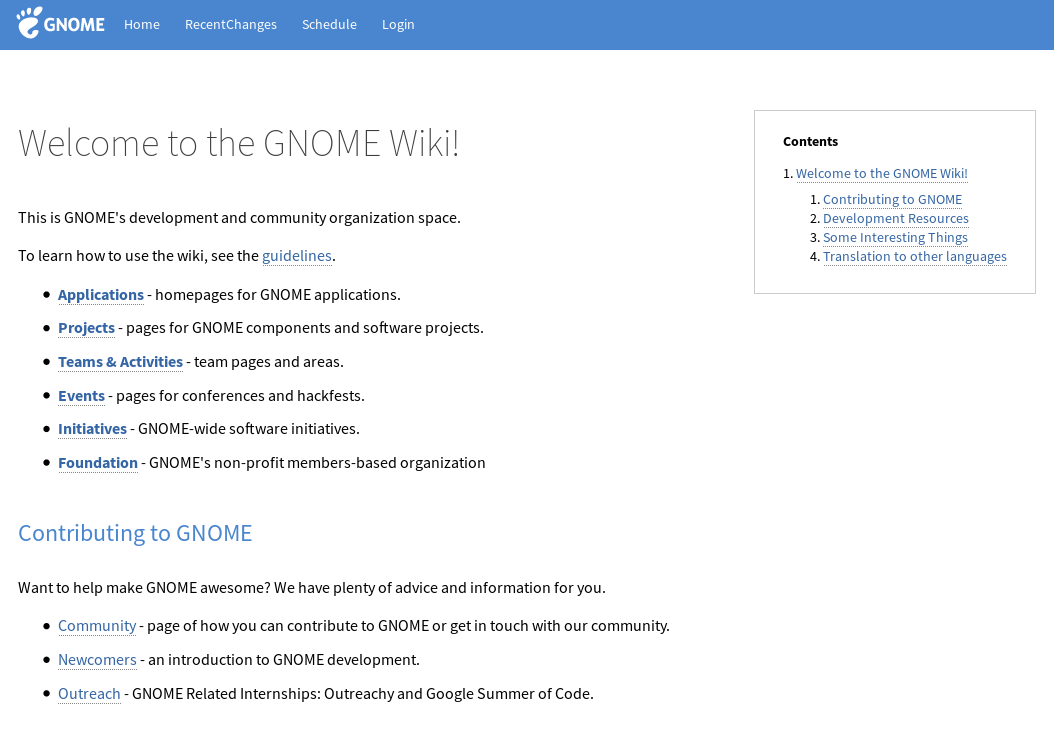
\includegraphics[width=15cm]{images/wiki_gnome_org.png}
\end{figure}

\begin{figure}[p]
  % from: https://git.gnome.org
  \caption{\label{figure_cgit} Interface git du projet GNOME}
  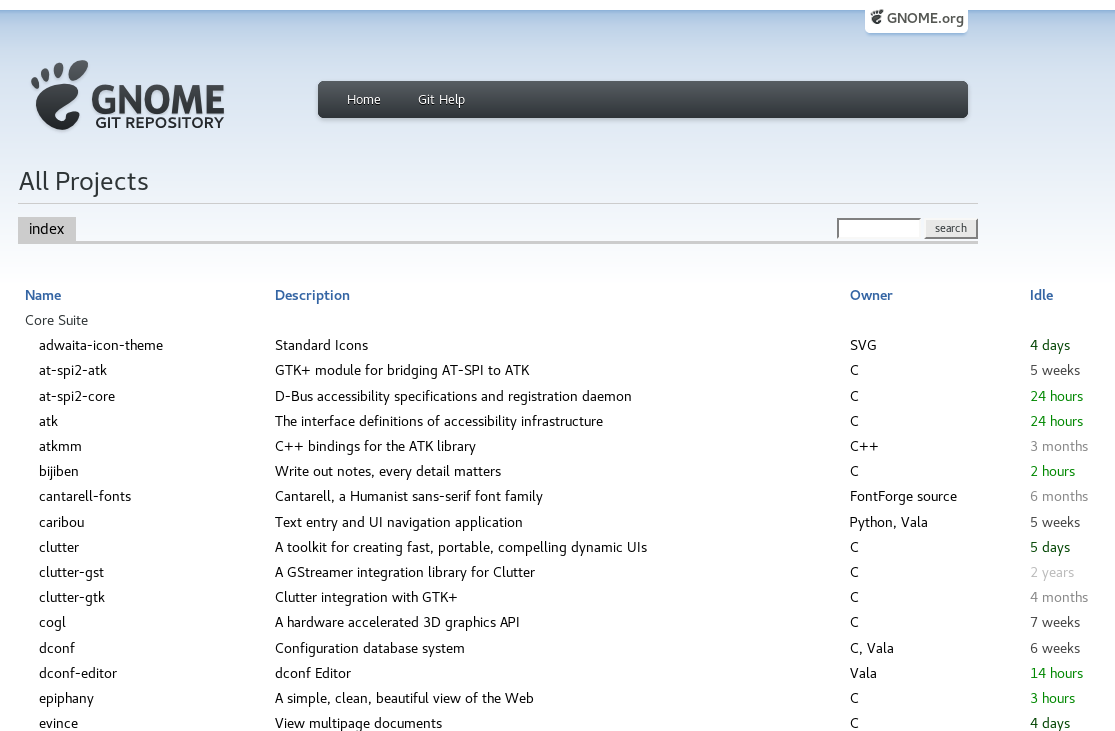
\includegraphics[width=15cm]{images/git_gnome_org.png}
\end{figure}

\begin{figure}[p]
  % from: https://gitlab.gnome.org
  \caption{\label{figure_gitlab} Le gitlab du projet GNOME}
  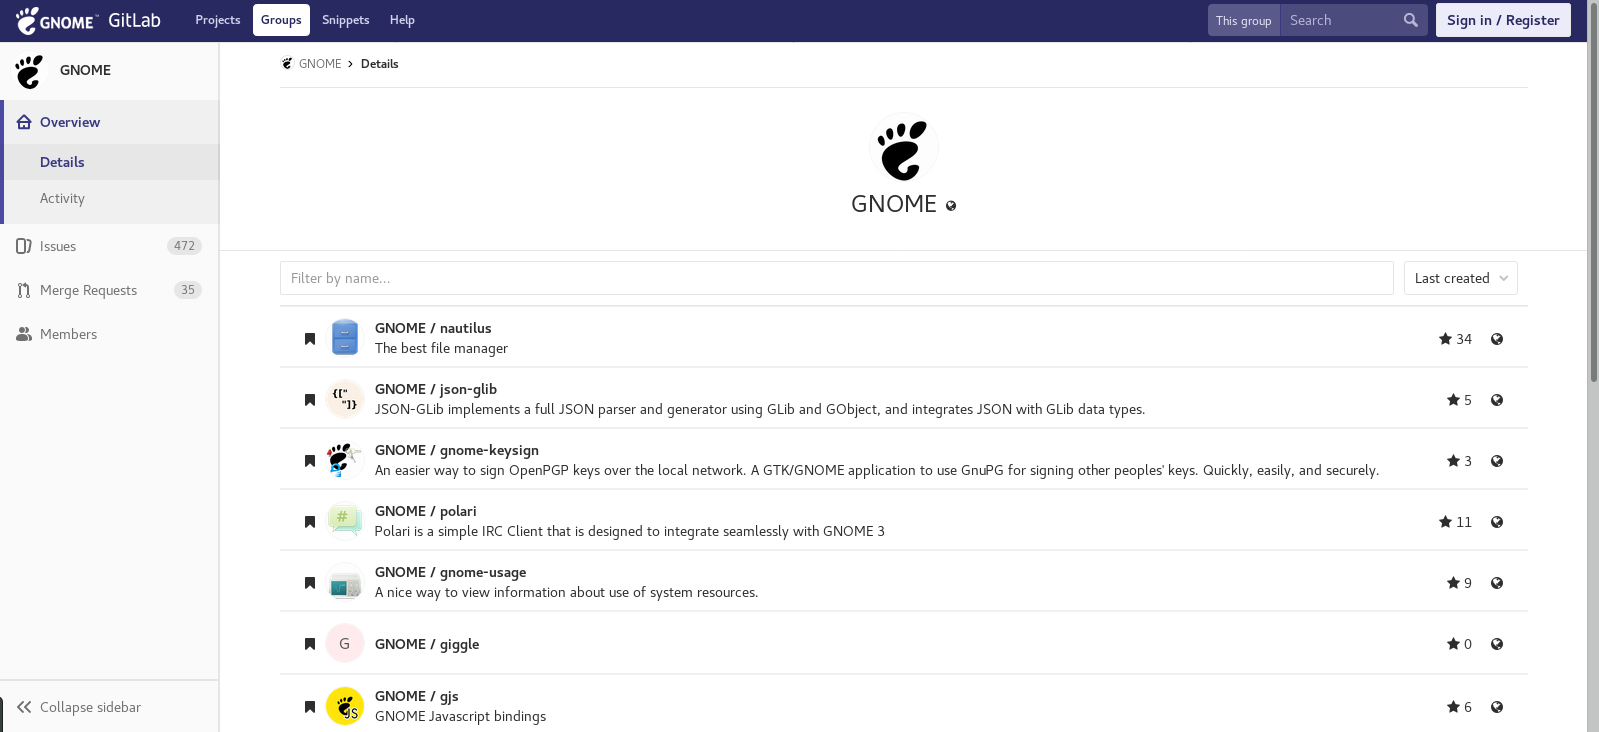
\includegraphics[width=15cm]{images/gitlab_gnome_org.png}
\end{figure}

\chapter{Patchs} 
% PA: Utile ? 

\end{document}
